\chapter{関連研究}
\label{chap:previousworks}
本章では\secref{sec:generate_animation}で音からアニメーションを自動生成する研究を紹介し,\secref{sec:generate_}でアニメーションから音を自動生成する研究を紹介する.
\secref{sec:synchronization}では音とアニメーションを同期させる研究を紹介し,最後に\secref{sec:compere}にて本研究の新規性を述べる.

\section{音からアニメーションを自動生成する研究}\label{sec:generate_animation}
音とアニメーションを同期させることを目的として,音からアニメーションを自動生成する研究は多く存在している.\\
\indent
物が落下するアニメーションを生成するには,物の落下音と物が落下するタイミングを1つ1つ合わせる必要がある.
Langloisら\cite{IFA}は,それらを正確に合わせるために,物が落下する音が収録されている音源から,物が落下するアニメーション\ref{fig:IFA}を自動生成する手法を提案した.
\begin{figure}[h]
	\centering
	
\includegraphics[width=15cm]{fig/chap2/IFA.eps}
	\caption{落下アニメーションの自動生成}
	\label{fig:IFA}
\end{figure}

\indent
キャラクタの口の動きと音声を合わせる,リップシンクも難しい課題となっている.
キャラクタの口の動きに合わせて後から音声を録音するアフレコは比較的容易であるが,音声から,その言葉を発している口元のアニメーションの生成は,言葉と口の形,そして発するタイミングと口の動きを合わせる必要があり,ひじょうに難易度が高い.
そこで,Edwardsら\cite{JALI}は,台詞が収録されている音源および台詞が記載されているテキストファイルを入力すると,その台詞を話している口元のアニメーション\ref{fig:JALI}を自動生成する手法を提案した.
本手法では,顎と唇のみを制御することにより,自然な口元のアニメーションを自動生成している.更に,後から表情を編集することが可能となっているため,最終的には自然な表情のアニメーションが完成する.
\begin{figure}[h]
	\centering
	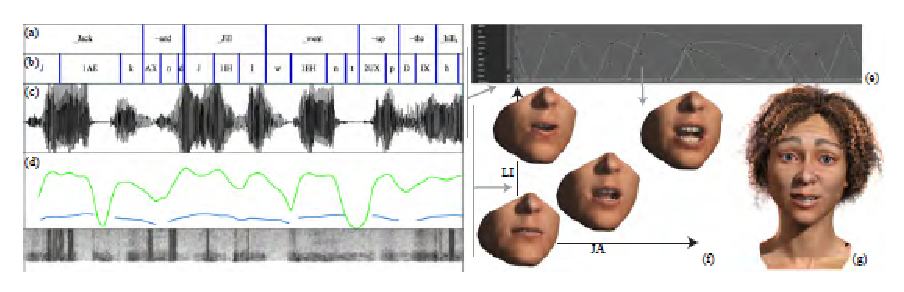
\includegraphics[width=15cm]{fig/chap2/JALI.eps}
	\caption{口元アニメーションの自動生成}
	\label{fig:JALI}
\end{figure}

\section{アニメーションから音を生成する研究}\label{sec:generate_sound}

\section{音とアニメーションを同期させる研究} \label{sec:synchronization}

\section{本研究との関連}\label{sec:compere}



